%!TEX program=xelatex

\documentclass[11pt]{ctexart}  
\usepackage[top=2cm, bottom=2cm, left=2cm, right=2cm]{geometry}  
\usepackage{algorithm}  
\usepackage{algorithmicx}  
\usepackage{algpseudocode}  
\usepackage{amsmath}  
\usepackage{graphicx}
\usepackage{amsmath}
\usepackage{amssymb}
\usepackage{enumerate}
\usepackage{booktabs}

\floatname{algorithm}{算法}
\renewcommand{\algorithmicrequire}{\textbf{输入:}}  
\renewcommand{\algorithmicensure}{\textbf{输出:}} 

\title{密码学实验报告7}
\author{张天辰 17377321}

\makeatletter
\newenvironment{breakablealgorithm}
  {% \begin{breakablealgorithm}
   \begin{center}
     \refstepcounter{algorithm}% New algorithm
     \hrule height.8pt depth0pt \kern2pt% \@fs@pre for \@fs@ruled
     \renewcommand{\caption}[2][\relax]{% Make a new \caption
       {\raggedright\textbf{\ALG@name~\thealgorithm} ##2\par}%
       \ifx\relax##1\relax % #1 is \relax
         \addcontentsline{loa}{algorithm}{\protect\numberline{\thealgorithm}##2}%
       \else % #1 is not \relax
         \addcontentsline{loa}{algorithm}{\protect\numberline{\thealgorithm}##1}%
       \fi
       \kern2pt\hrule\kern2pt
     }
  }{% \end{breakablealgorithm}
     \kern2pt\hrule\relax% \@fs@post for \@fs@ruled
   \end{center}
  }
\makeatother

\begin{document}
\maketitle{}



\section{大数运算——C++语言实现}
\subsection{大数运算算法} % (fold)
首先,为了存储大数又兼顾效率,采用如下的数据结构:将大整数切割成一段一段,即每次把大数模$10^9$的结果存储在列表中,再把大数除以$10^9$。这样,它就会被9位9位存储起来。

在完成了对大数的构造之后,就需要进行各种关系的重写,并且重载运算符。对于大小关系,只需要比较两个数的分段数量,如果相同再逐个比较每个分段即可。

对于大数加法,只需要从对齐的低位分段开始逐段相加即可,每次相加之后判断进位。对于大数减法,也是类似的,只不过逐段相减之前要先判断能不能减,如果不能减则要向高位借位。对于乘法,需要按照类似竖式计算的方法进行逐段乘法和移位相加。以上三种算法都基于竖式计算,比较直观。

除法计算如果直接采用仿照竖式的方法,效率较低。我参考了网上的一种高效算法。首先,有这样的结论:
$$\frac{\overline{a_{n-1}a_{n-2}\cdots a_{1}a_{0}}}{\overline{b_{n-1}b_{n-2}\cdots b_{1}b_{0}}} \leqslant \frac{\overline{a_{n-1}a_{n-2}\cdots a_{i}}}{\overline{b_{n-1}b_{n-2}\cdots b_{i}}}$$

于是,可以通过取被除数和除数的高位来估计商,并根据这个估计的商更新被除数,通过计算逼近实际的商。具体算法如下,对于$A/B$有:
\begin{enumerate}[1]
    \item 计算$C_0 = A / B$,得到商$V_0$。令$A_1 = B * V_0 - A$。
    \item 计算$C_1 = A_1 / B$,得到商$V_1$。令$A_2 = B * V_1 - A_1$。
    \item $\cdots$
    \item 计算$C_n = A_n / B$,得到商$V_n$。$V_n * B - A = 0$。
\end{enumerate}
则实际的商约为$V_0 - V_1 + V_2 \cdots$。实际上,真实的商比上述估计值小一或相等,只需估计后进行调整、验证即可。对于大数的除法,只要先模仿竖式计算进行,在每一步的除法中应用上述算法即可。

关于模幂运算,只是把之前写过的快速幂算法搬过来即可。因为重载了运算符,所以几乎不用做改动。
% subsection 查找表优化简介 (end)
\subsection{算法实现} % (fold)
我写的实际算法是类方法,这里变换成普通函数。
\begin{breakablealgorithm} 
\caption{大整数比较}
\begin{algorithmic}[1] %每行显示行号  
    \Function{compare}{$a, b$}
    \State $len1 \gets a.data.size()$
    \State $len2 \gets b.data.size()$
    \If {$len1 \neq len2$}
        \State \Return $len1 > len2 ? 1 : -1$
    \EndIf
    \For {$cmp$ from $len1 - 1$ to $0$}
        \If {$a.data[cmp] \neq b.data[cmp]$}
            \State \Return $a.data[cmp] > b.data[cmp] ? 1 : -1$
        \EndIf
    \EndFor
    \State \Return $0$
    \EndFunction
\end{algorithmic}
\end{breakablealgorithm}
\begin{breakablealgorithm} 
\caption{大整数加法}
\begin{algorithmic}[1] %每行显示行号  
    \Function{add}{$a, b$}
    \State $len1 \gets a.data.size()$
    \State $len2 \gets b.data.size()$
    \State $result \gets null$
    \For {$cnt$ from $0$ to $min{len1, len2}$}
        \State $result$写入$a.data[cnt]+b.data[cnt]+carry$
        \State 计算进位$carry$
    \EndFor
    \For {$cnt$ from $min{len1, len2}$ to $max{len1, len2}$}
        \State $result$写入$max{a, b}[cnt]+carry$
        \State 计算进位$carry$
    \EndFor
    \State $result$写入余下的$carry$。
    \State \Return $result$
    \EndFunction
\end{algorithmic}
\end{breakablealgorithm}
\begin{breakablealgorithm} 
\caption{大整数减法}
\begin{algorithmic}[1] %每行显示行号  
    \Function{subtract}{$a, b$}
    \State 保证$a >geqslant b$,否则交换$a, b$
    \State $len1 \gets a.data.size()$
    \State $len2 \gets b.data.size()$
    \State $result \gets null$
    \For {$cnt$ from $0$ to $len2$}
        \If {$a.data[cnt] < b.data[cnt] + carry$}
            \State $result$写入$a.data[cnt]-b.data[cnt]-carry+MAX$
            \State $carry = 1$
        \Else
            \State $result$写入$a.data[cnt]-b.data[cnt]-carry$
            \State $carry = 0$
        \EndIf
    \EndFor
    \For {$cnt$ from $len2$ to $len1$}
        \If {$a.data[cnt] < carry$}
            \State $result$写入$a.data[cnt]-carry+MAX$
            \State $carry = 1$
        \Else
            \State $result$写入$a.data[cnt]-carry$
            \State $carry = 0$
        \EndIf
    \EndFor
    \State \Return $result$
    \EndFunction
\end{algorithmic}
\end{breakablealgorithm}
\begin{breakablealgorithm} 
\caption{大整数乘法}
\begin{algorithmic}[1] %每行显示行号  
    \Function{multiply}{$a, b$}
    \State $len1 \gets a.data.size()$
    \State $len2 \gets b.data.size()$
    \State 保证$a >geqslant b$,否则交换$a, b$
    \For {$cnt2$ from $0$ to $len2$}
        \State 在$temp$低位写入$cnt2$组0,用于移位
        \State $b.data[cnt2]$依次乘$a.data$各组,写入$temp$,计算进位
        \State 将$temp$结果写入$result$
    \EndFor
    \State \Return $result$
    \EndFunction
\end{algorithmic}
\end{breakablealgorithm}
\begin{breakablealgorithm} 
\caption{大整数除法}
\begin{algorithmic}[1] %每行显示行号  
    \Function{divide}{$a, b$}
    \State $len1 \gets a.data.size()$
    \State $len2 \gets b.data.size()$
    \State 保证$a >geqslant b$,否则返回$0$
    \State 选出$a$的高$len2-1$位写入$beDivide$
    \For {每次从$a$中选出一块拼接$beDivide$和$b$进行除法}
        \State $value \gets$\Call{partDivide}{$beDivide, b$}
        \State $beDivide \gets beDivide - b * value$
        \State $value$写入$result$低位
    \EndFor
    \State \Return $result$
    \EndFunction
    \Function{partDivide}{$beDivide, b$}
    \State $temp1 \gets partDivide$
    \State $temp2 \gets b$
    \While{$temp1 \geqslant temp2$}
        \If{$len(temp1.data) > len(temp2.data)$}
            \State $temp1$取高2组,$temp2$取高1组除
        \Else
            \State $temp1, temp2$取高2组除;如果不足就取1组
        \EndIf
        \State 更新$temp1$
        \State 将商按照正确的符号写入$result$
    \EndWhile
    \State 调整$result$使其正确
    \State \Return $result$
    \EndFunction
\end{algorithmic}
\end{breakablealgorithm}

取模操作实际上就是除法、减法和乘法的组合,这里略去。此外,模幂运算复用之前实验的快速幂算法逻辑,只不过在另一种语言上重写。因为重载了运算符,改动并不大,这里也从略。
% subsection 算法实现 (end)
\subsection{算法测试} % (fold)
我没有测试加法减法除法,因为这些都可以在乘法和模幂运算中得到测试。这里的测试数据都是我在做完RSA实验之后从里面选取的数据。
\begin{enumerate}
    \item 乘法测试

    这里采用了RSA密钥生成程序给出的两个大素数$p, q$。它们相乘达到了1024bit。输出第一行为运行时间,可以看出速度相当快;第二行为其与正确答案是否相等的比较,为1代表相同,结果正确。
    \begin{figure}[htbp]
    \centering
    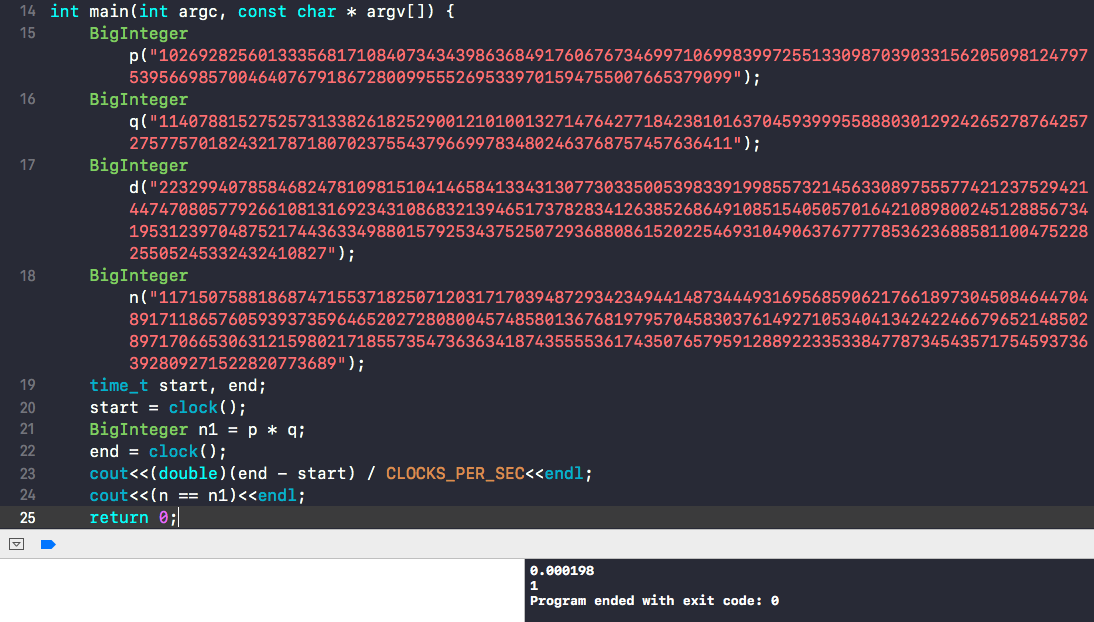
\includegraphics[height=9.95cm,width=17.50cm]{test_multi.png}
    \caption{大数乘法测试}
    \label{test_multi}
    \end{figure}

    \item 模幂测试

    同样采用RSA解密的中间数据。其中$n$为1024bit,其余的$c,d$大小相仿,在1000bit以上。由代码可以看出,运行时间约5秒。我在python下对同样的数据进行了测试。首先可以证明结果的正确性,其次,python对这样的数据几乎是在一瞬之间给出答案,说明我的代码在除法上与python还有很大的差距。
    \begin{figure}[htbp]
    \centering
    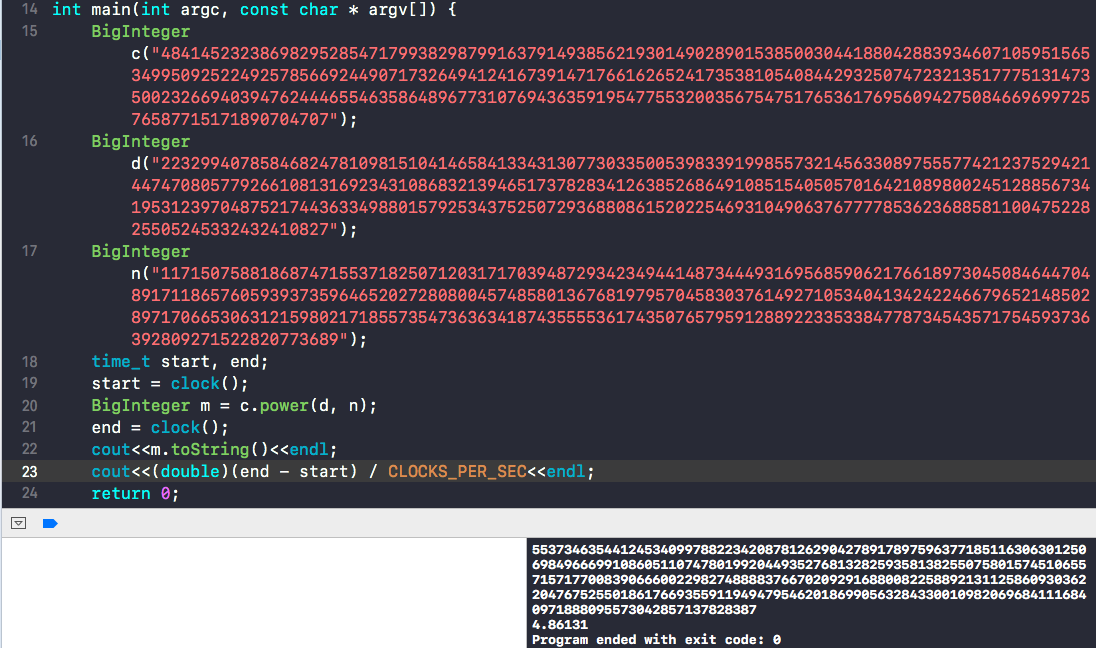
\includegraphics[height=10.37cm,width=17.54cm]{test_power.png}
    \caption{大数模幂测试}
    \label{test_power}
    \end{figure}

\end{enumerate}

\section{RSA加解密——Python实现} % (fold)
\subsection{RSA逻辑与OAEP填充} % (fold)
RSA是基于大整数分解难题的公钥算法。OAEP又称最佳非对称加密填充,是一种利用掩膜生成函数和哈希函数构造的填充方法,可以很好地防止选择密文攻击。相对RSA破解的难度而言,进行OAEP填充是有意义的。关于OAEP的填充算法,具体可以参见RSA标准。

RSA算法的基本内容如下:选取两个大素数$p, q$,计算$n = pq$,$\phi(n) = (p-1)(q-1)$。选取$e$满足$\gcd(e, \phi(n)) = 1$,及$d$为$e$模$\phi(n)$的逆。把$e, n$作为公钥,$p, q, d$作为私钥。

加密过程为$c = m^e \mod n$,解密过程为$m = c^d \mod n$。其中解密过程可以利用中国剩余定理优化如下:要解$c^d \mod n$即要解
$$x \equiv c^d \mod p \quad \quad x \equiv c^d \mod q$$
设
$$r1 \equiv d \mod (p-1) \quad \quad r2 \equiv d \mod (q-1)$$
则就转化为解
$$x \equiv c^{r1} \mod p \quad \quad x \equiv c^{r2} \mod q$$
利用中国剩余定理可求解。
% subsection rsa逻辑与oaep填充 (end)
\subsection{算法实现} % (fold)
\begin{enumerate}
    \item 密钥生成

    密钥生成可以单独进行。为了后续计算、填充的方便,这里保证$n$为1024bit。具体实现方式如下:

    满足长度为1024bit的数范围如下:$[2^{1023}, 2^{1024}-1]$,因此$p, q$的范围就是$[2^{\frac{1023}{2}}, 2^{512})$。$2^{\frac{1023}{2}} < 2^{511} * 1.5 = 2^{511} + 2^{510}$。

    为了保证在$p, q$都是奇数的时候再进行素性检验,可以将$p, q$的生成方式变为$2k+1$的形式。将上述范围的2的幂次减1,就是$k$的范围。$p, q$重合或者$pq>2^1024$的概率太小,忽略不计。

    \begin{breakablealgorithm} 
    \caption{RSA密钥生成}
    \begin{algorithmic}[1] %每行显示行号  
        \Function{generateKey}{}
        \State $p \gets $\Call{generatePrime}{}
        \State $q \gets $\Call{generatePrime}{}
        \State $n \gets p * q$
        \State $\phi \gets (p-1)*(q-1)$
        \State $e \gets $\Call{randint}{$3, \phi - 1$}直到$\gcd(e, \phi) = 1$
        \State $d \gets $\Call{rev}{$e, \phi$}
        \State 分别写公钥文件和私钥文件
        \EndFunction
        \Function{generatePrime}{}
        \While {1}
            \State $temp \gets$\Call{randint}{$2^{510} + 2^{509}, 2^{511}$}
            \State $p \gets 2*temp+1$
            \If {\Call{MillerRabin}{$p$}}
                \State \Return $p$
            \EndIf
        \EndWhile
        \EndFunction
    \end{algorithmic}
    \end{breakablealgorithm}
    \item OAEP填充

    实在没什么特别的地方,无非是按照标准给出的算法做。这里给出流程图。解码时从$maskedDB$通过$MGF$及$maskedSeed$获得$seed$之后就显然了。
    \begin{figure}[htbp]
    \centering
    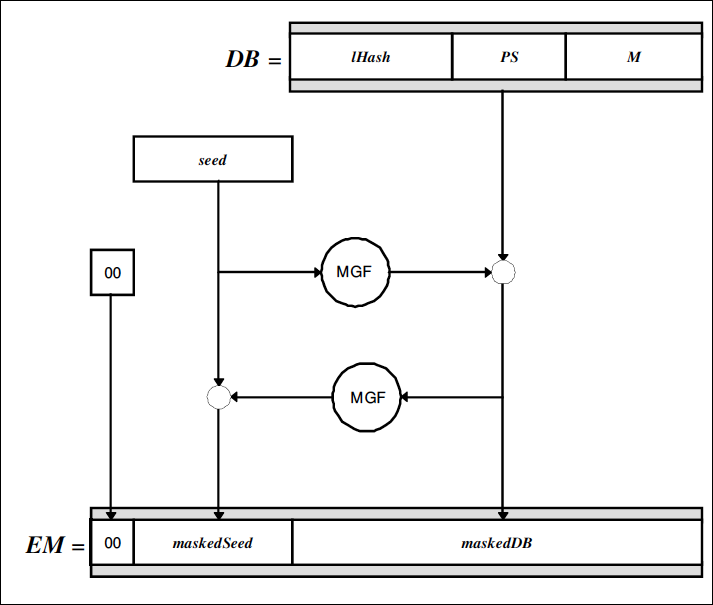
\includegraphics[height=9.08cm,width=10.67cm]{OAEP.png}
    \caption{OAEP流程}
    \label{update}
    \end{figure}
    \item MGF函数

    同样也是按照标准给出的算法逐步实现。
    \item RSA加解密

    首先,因为我在OAEP里的hash函数使用了sha-256,根据OAEP编码的计算规则和范围,将明文60字节分组比较恰当。把文件读入后按照60字节分组,并且在最后进行填充。填充规则为填充若干个0,并在最后一个字节写入填充的0的个数。

    \begin{breakablealgorithm} 
    \caption{RSA}
    \begin{algorithmic}[1] %每行显示行号  
        \Function{encrypt}{$plainList$}
            \For{$p \in plainList$}
                \State $plain \gets$对$p$进行OAEP编码
                \State $cipherList.append(plain^{e} \mod n)$
            \EndFor
        \EndFunction
        \Function{decrypt}{$cipherList$}
            \State 读文件得到$p, q, d$
            \For {$c \in cipherList$}
                \State $r1 \gets d \% (p-1)$
                \State $r2 \gets d \% (q-1)$
                \State $p1 \gets$\Call{modPower}{$c, r1, p$}
                \State $p2 \gets$\Call{modPower}{$c, r2, q$}
                \State $plain \gets$\Call{CRT}{$[p1, p2], [p, q], n$} 
                \State $temp \gets$对$plain$进行OAEP解码
                \State $plainList.append(temp)$
            \EndFor
        \EndFunction
    \end{algorithmic}
    \end{breakablealgorithm}
\end{enumerate}
% subsection 算法实现 (end)
\subsection{测试结果} % (fold)
我实现了一个简单的GUI界面用于加密和解密,选取了一张约400KB的图片进行加密,再进行解密。如图\ref{test_rsa},右边为加密后的文件,左边为解密得到的原文件,从预览图就可看出成功解密。图\ref{test_rsa}还显示了GUI界面的设计。加密时只需点击生成密钥就可生成公私钥对,解密时把私钥文件和代码放在同一文件夹即可。唯一的不足是代码执行速度太慢,加密这个文件用了约40s,解密用了约30s,需要后期的进一步优化。
\begin{figure}[htbp]
    \centering
    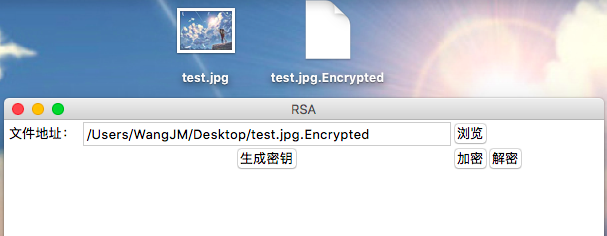
\includegraphics[height=4.72cm,width=12.14cm]{test_rsa.png}
    \caption{RSA测试}
    \label{test_rsa}
    \end{figure}
% subsection 测试结果 (end)
% section rsa加解密_python实现 (end)
\section{简单背包密码体制} % (fold)
\subsection{背包密码体制及其攻击} % (fold)
背包密码体制的私钥为一个超递增背包序列。根据模数$m$和乘数$w$,其中$\gcd (m, w) = 1$,可以构造公钥:对私钥里的每个$r$,对应公钥的权重为$p \equiv rw \mod w$。利用公钥作为背包对消息加密得到密文。将密文在模$m$下乘以$w$关于$m$的逆,再解超递增背包问题就可以得到明文。

背包密码体制的攻击为只要选出$w, m$使得能把公钥背包变成超递增背包,就可以用那个背包和选出的$w, m$解密。奇怪的地方在于,我用这种方法编写的程序有可能得到错误的明文,初步猜测是$m$太小导致。
% subsection 背包密码体制及其攻击 (end)
\subsection{算法实现} % (fold)
\begin{breakablealgorithm} 
    \caption{背包密码}
    \begin{algorithmic}[1] %每行显示行号  
        \Function{generateKey}{$len$}
            \State 生成长度为$plain$二进制长度的超递增背包,为私钥 
            \State 随机产生$m, w$使得$\gcd (w, m) = 1$
            \State 私钥的每一项模$m$乘$w$,得到公钥
        \EndFunction
        \Function{encrypt}{$plain$}
            \State 用公钥背包加密$plain$的二进制串
        \EndFunction
        \Function{decrypt}{$cipher$}
            \State $c \gets cipher * \overline{w} \mod m$
            \State 用私钥背包解$c$
        \EndFunction
    \end{algorithmic}
    \end{breakablealgorithm}
    \begin{breakablealgorithm} 
    \caption{背包密码攻击}
    \begin{algorithmic}[1] %每行显示行号  
        \Function{attack}{$pub, cipher$}
            \State 随机生成$m, w$使得$\gcd (m, w) = 1$
            \State 如果公钥模$m$乘$\overline{w}$没得到超递增背包,就返回上一步
            \State 用得到的私钥进行解密$cipher$
        \EndFunction
    \end{algorithmic}
    \end{breakablealgorithm}
% subsection 算法实现 (end)
\subsection{测试样例} % (fold)
测试使用的数据是数字,可以自动生成公私钥加密或解密。没有写成加密解密分开实现的形式,将进行改进。
\begin{figure}[htbp]
    \centering
    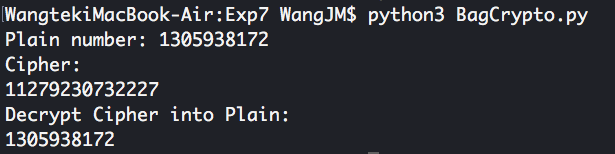
\includegraphics[height=3.08cm,width=12.30cm]{Bag.png}
    \caption{背包密码测试}
    \label{bag}
    \end{figure}

攻击算法只能解决长度为9以下的背包,因为使用了随机数所以耗时不等,奇怪的是可能解密出错,正在研究。
\begin{figure}[htbp]
    \centering
    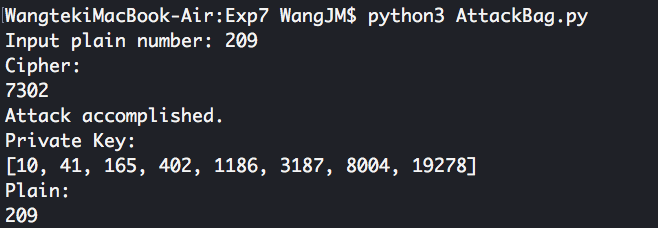
\includegraphics[height=4.56cm,width=13.16cm]{Attack.png}
    \caption{背包密码攻击测试}
    \label{attack}
    \end{figure}
% subsection 测试样例 (end)
% section 简单背包密码体制 (end)
\end{document}